\subsection{Проектирование функциональных требования}

Функционал программного средства – ключевая точка разработки программного средства, составляющей которого являются алгоритмы.
В связи с этим, программное средство {\taskNameFull} должно обладать некоторыми алгоритмами:
\begin{itemize}
    \item алгоритм создания JWT токена;
    \item алгоритм сохранения файла в облачное хранилище;
    \item алгоритм отправки уведомления в систему логирования;
\end{itemize}

\subsubsection{Алгоритм создания JWT токена}

JWT токен \cite{jwtDocs} -- это JSON Web Token, который используется для передачи информации между клиентом и сервером в виде JSON объекта.
Алгоритм создания JWT токена представлен на рисунке \ref{fig:jwt}.

\begin{figure}[ht]
    \centering
    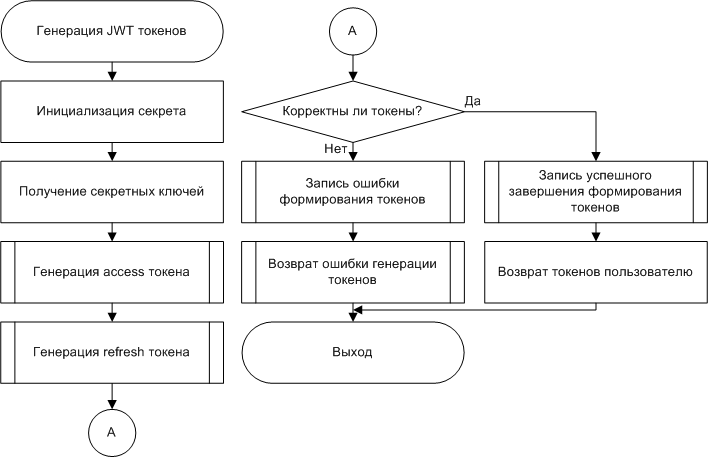
\includegraphics[width=0.80\linewidth]{\commonSecPathPrefix/sec_2/content/jwt.png}
    \caption{Алгоритм создания JWT токена}
    \label{fig:jwt}
\end{figure}

JWT токен состоит из трех частей: заголовка, полезной нагрузки и подписи. Заголовок содержит информацию о типе токена и 
алгоритме подписи. Полезная нагрузка содержит информацию о пользователе и сроке действия токена. Подпись используется для проверки 
целостности токена и его подлинности.

Access токен -- это токен, который используется для доступа к защищенным ресурсам.
Refresh токен -- это токен, который используется для получения нового JWT токена, когда срок действия старого токена истек.
Refresh токен имеет больший срок действия, чем Access токен.

\subsubsection{Алгоритм сохранения файла в облачное хранилище}

Облачное хранилище -- это сервис, который позволяет хранить данные в интернете и получать к ним доступ из любой точки мира.
Облачное хранилище позволяет хранить данные в защищенном виде и обеспечивает доступ к ним только авторизованным пользователям.

Алгоритм сохранения файла в облачное хранилище представлен на рисунке \ref{fig:save_file}.

\begin{figure}[ht]
    \centering
    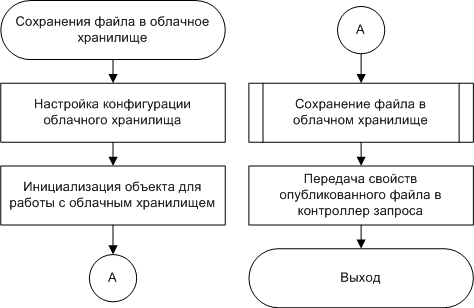
\includegraphics[width=0.60\linewidth]{\commonSecPathPrefix/sec_2/content/cloud.png}
    \caption{Алгоритм сохранения файла в облачное хранилище}
    \label{fig:save_file}
\end{figure}

Алгоритм сохранения файла в облачное хранилище начинается с инициализации необходимых компонентов: имя облачного хранилища,
API ключ и API секрет. После этого инициализируется объект, через который будет происходить взаимодействие с облачным хранилищем.
В объекте настраиваются параметры облачного хранилища: папка и формат файлов. После этого используя внутренние библиотеки языка
программирования можно выполнить функцию для загрузки файла в облако. Результат работы это свойства опубликованного файла, которые
передаются обработчику запроса для дальнейшего взаимодействия.

\subsubsection{Алгоритм отправки уведомления в систему логирования}

Система логирования -- это система, которая позволяет отслеживать события, происходящие в программном обеспечении.
Система логирования позволяет сохранять информацию о событиях, происходящих в программном обеспечении, и предоставляет возможность
анализировать эту информацию.
Алгоритм отправки уведомления в систему логирования представлен на рисунке \ref{fig:log}.

\begin{figure}[ht]
    \centering
    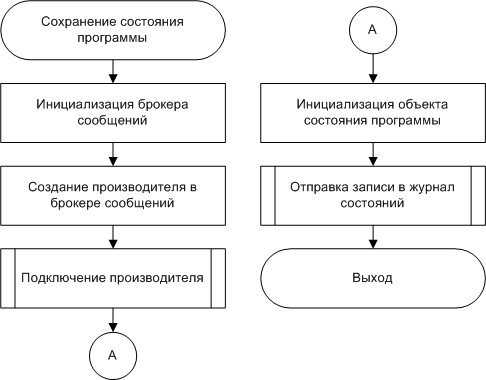
\includegraphics[width=0.60\linewidth]{\commonSecPathPrefix/sec_2/content/logs.png}
    \caption{Алгоритм отправки уведомления в систему логирования}
    \label{fig:log}
\end{figure}

Перед началом работы необходимо инициализировать брокер сообщений и создать производителя для генерации нового состояния в журнале
событий программного средства. Далее, при возникновении нового сообщения запускается производитель и формируется объект, который хранит
текущее состояние системы. Остаётся только создать событие в брокере через производителя и передать новое сообщение.